\documentclass[conference]{IEEEtran}
\IEEEoverridecommandlockouts
% The preceding line is only needed to identify funding in the first footnote. If that is unneeded, please comment it out.
\usepackage{cite}
\usepackage{amsmath,amssymb,amsfonts}
\usepackage{algorithmic}
\usepackage{graphicx}
\usepackage{textcomp}
\usepackage{xcolor}
\usepackage{minted}
\usepackage{hyperref}
\usepackage{multirow}
\usepackage{soul}

% \def\BibTeX{{\rm B\kern-.05em{\sc i\kern-.025em b}\kern-.08em
%     T\kern-.1667em\lower.7ex\hbox{E}\kern-.125emX}}

% Custom Commands
\newcommand{\ie}{\textit{i.e.},\ }
\newcommand{\eg}{\textit{e.g.},\ }
\newcommand{\etal}{\textit{et al.} }
\newcommand{\etc}{{\em etc.}}

\newcommand{\latif}[1]{\textcolor{blue}{\textit{#1}}}
\newcommand{\joanna}[1]{\textcolor{red}{\textit{#1}}}
\usepackage{enumitem}           % for numbered enumerations and margins
\usepackage[most]{tcolorbox}
\usepackage[parfill]{parskip}

\newcommand{\complexity}[1]{$\mathcal{O}(#1)$}


\tcbset{
  parskip/.style={
    before={\par\pagebreak[0]\parindent=0pt},
    after={\parfillskip=0pt\par},
  },
}
\newtcolorbox{resultbox}[1][]{%
    colback=black!5,
    colframe=black!5,
    notitle,
    sharp corners,
    borderline west={2pt}{0pt}{red!80!black},
    enhanced,
    breakable,
    boxsep=0pt,
    left=8pt,right=2pt,top=2pt,bottom=2pt,
    }
\newcommand{\rques}[1]{  
\begin{tcolorbox}[enhanced jigsaw,drop shadow=black!50!white,colback=white,left=2pt,right=2pt,top=2pt,bottom=2pt]
#1
\end{tcolorbox}
}

\pagenumbering{arabic}
\usepackage[utf8]{inputenc}
\usepackage{booktabs}
%*************************************************************
% BEGIN CUSTOMIZATIONS FOR MINTED PACKAGE                    *
%*************************************************************
% http://tug.ctan.org/macros/latex/contrib/minted/minted.pdf *
%*************************************************************
\usemintedstyle{tango}
\newminted{python}{frame=single,linenos,numbersep=3pt,fontsize=\scriptsize,xleftmargin=7pt}
\definecolor{codebg}{rgb}{0.99,0.99,0.99}
\definecolor{hiliteColor}{rgb}{1,0.92549019607,0.6}
\definecolor{tainted}{rgb}{0,1,1}
\newcommand{\highlight}[1]{\colorbox{hiliteColor}{#1}}
\DeclareRobustCommand{\hlcyan}[1]{{\sethlcolor{tainted}\hl{#1}}}
\DeclareRobustCommand{\hlred}[1]{{\sethlcolor{red!25}\hl{#1}}}
\setlength\fboxsep{0.5pt}
\newcommand{\PythonCode}[3]{%
\inputminted[%
  highlightlines={#2},
  highlightcolor=hiliteColor,
  escapeinside=||,
  framerule=0.5pt,
  bgcolor=white,
  numbersep=2pt,
  framesep=15pt,
  firstnumber={#3}
]{python}{#1}}



\newmintinline{java}{fontsize=\scriptsize}

\newminted[JavaSourceCode]{java}{
    labelposition=topline,
    frame=single,
    numbersep=2pt,
    fontsize=\scriptsize,
    xleftmargin=5pt,
    framerule=0.5pt,
    linenos, rulecolor=\color{gray!60}
}


% CSE 326 ISD Group B2 : 3 \\
% Roll: 1805112, 1805110, 1805115, 1805113, 1805092, 1805116

\begin{document}

\title{Usability Analysis of Bangladesh e-Passport Portal: A Study on Public Software Project}

\author{\IEEEauthorblockN{Md. Asif Haider, Anika Monir}
\IEEEauthorblockA{Department of Computer Science and Engineering
}
\IEEEauthorblockA{Bangladesh University of Engineering and Technology
}}


\maketitle
% \begingroup\renewcommand\thefootnote{\textsection}
% \footnotetext{These authors equally contributed to this work.}
% \endgroup
\thispagestyle{plain}
\pagestyle{plain}
\begin{abstract}
Public software projects play a significant role in making the lives of the citizens of a country much easier by providing public services at a large scale. The E-passport portal is such a website with a huge number of clients based in the context of Bangladesh. Hence, studying the web application from a Software Engineering and System Design point of view is crucial, especially when there is a scope for improving user experience. In this study, we analyze the web application and its features based on public opinion and first-hand testing. Finally, we suggest spot-on recommendations to improve the project further.
\end{abstract}

\begin{IEEEkeywords}
% code generation, complexity, transformer, zero-shot prompting,  pre-trained model, GitHub copilot
public software projects, questionnaire survey, e-passport, user experience
\end{IEEEkeywords}

\section{Introduction}\label{sec:intro}
Bangladesh e-Passport Portal \footnote{\url{https://www.epassport.gov.bd/landing}}, the subject web application for our study, is one of the most notable publicly available software projects in Bangladesh. The portal is currently being used to serve the citizens of the country, offering both registration and renewal of an electronic passport (e-passport). The e-passport portal was introduced as a part of the E-passport and Automated Border Control Management project, jointly designed and developed by the German identity service provider company Veridos GmBH, and the Department of Passport and Immigration of the People’s republic of Bangladesh with assistance from the Bangladesh Army and the Security Services Division of the Home Ministry \cite{c21}. The project, in its all, was implemented at an approximate cost of 4569 crore taka. The online application portal enjoyed its pilot deployment phase starting in January 2020 \footnote{\url{http://www.dip.gov.bd/site/view/innovation/Piloting\%20Project}}, and finally was adopted country-wide in the middle of the same calendar year. 

The services provided by the portal can be categorized into 2 major sections. First comes the online application that the user has to fill up completely to apply for a passport. It also contains a status-checking dashboard to track and notify about the progress of passport processing. It contains an urgent application section to serve emergency cases. Moreover, the system incorporated an online payment platform to ease the fee payment process. Second, comes the assisting segment of the website. It is presented with the information section consisting of the step by step instructions, payment options, frequently asked questions (FAQs), notices, and last but not the least, a user feedback system.

Being a significant example of one the most used public software projects in the country, the Bangladesh e-Passport Portal serves a massive amount of people every year, with a very high daily usage time and user load. Hence, we chose this website to analyze its functionality and performance from the eyes of a regular user. We collected user experience data to validate our analysis and to find new insights about the strong and weak features of the website as well.


% \input{Files/background}
% \input{Files/rquestions}

\section{Methodology}\label{sec:method}

The primary objective of our study was to critically study the e-Passport portal application from a Software Engineering and System Design point of view. The applied methodology was to test every feature of the website by hand, and report any issues found related to the user interface, technical performance, and informational clarity. Aside from using and testing it ourselves, we collected public opinions on the existing application through a carefully curated anonymous questionnaire survey distributed through public social media platforms. Hence, the analysis of our chosen application heavily relies on both personal and popular use-case scenarios and first-hand user experience. The goal of the experiment was to figure out both the positive and negative aspects of the website. Additionally, our target was to present appropriate recommendations based on both well-known software design principles and user feedback to improve the usability of the mentioned application. 

The participant group for the experiment can be divided into two types- the authors who used and tested the system on their own, and the survey participants who shared their own experiences while using the software. 

\subsection{Participant Group I}

The authors followed a common pattern to navigate through the website. We checked out each header section and the links inside those that direct to different web pages the website consists of. For each web page, we tested the functionality it provides. We filled up the forms and input boxes where needed, and studied the information and instructions shared by the system admins. While going through the system, we specifically looked for potential information gaps, technical and visual disturbance as well as performance compromise.

\subsection{Participant Group II}

After preparing a primary overview of the system's usability, we created a questionnaire survey to distribute among the mass public to gather more data on the user experience. The questionnaire contains 4 major sections in it which are as follows: Basic participant information, User interface, instructions, and technical feedback, Speed and performance feedback, Contact, and overall feedback. The detailed questionnaire can be found here \footnote{\url{https://forms.gle/6oEvZbymMfF7uzqq5}}. Based on the survey response, we validated our primary findings and found some new issues that we initially missed out on. Finally, we propose recommendations based on our overall findings from our experimental methods.
\section{Findings}
\label{sec:result}
\subsection{Primary Evaluation}

The first set of findings came directly from the testing performed by the authors. Initially, we found two problems regarding login and setting up a new account. While registering for the first time with an official departmental email (with .buet.ac.bd as the suffix), the input form showed an error. As it turned out, we could not proceed because some of the input fields got frozen. Changing the email input field to a regular email address solved this issue. Next while trying to perform a login, the website took an unusually high amount of time on average. 

To start with the web pages, we first landed on the homepage and navigated around it. It contained 7 header tabs constantly being displayed at the top of the webpage. Moving downwards, there were notice and news sections that contained hyperlinks to the latest notices sorted from the newest to the oldest order. There was a video demonstrating the history of passports and e-Passports in the country. There were also video links to e-Gate demonstrations.
Finally, there were 3 important additional links that direct to FAQs, About us, and Feedback pages. The FAQ page looked well-organized with multiple sections that answer some questions related together. The About us page provided a link to the website of the Department of Passport and Immigration. The feedback section, last updated on March 14, 2022, contained a link to the feedback form under the midterm evaluation of the whole project that asked for thoughtful feedback from the users to better improve the project.

Then we navigated through the tab titled ‘5 steps to e-Passport’ that enlists a brief set of necessary instructions in a step-by-step fashion. All the active 4 links were working fine, and the hyperlinks were marked differently for a better visual experience. The link from ‘Step 4’, listing the necessary documents to take with a user for biometric enrolment, had some information gap issues inside. Some contents of the document list were not clear enough. For example, it just mentioned one needs to bring NID and/or other identification documents. But in reality, one discovers that he/she needed to carry both original copies and photocopies of that document, after going to the passport office. The same problem was faced in the case of any previous passport, there was not anywhere mentioned on the website about bringing photocopies. This information should have been present in the system beforehand to improve user experience.

The information presented in the ‘Urgent Application’ tab looked quite well-organized and clear. There was a separate ‘Instructions’ tab that present important dos and don’ts regarding the application form. But it would have been better if those instructions were found alongside the application form itself. The ‘Passport fee’ tab contained information about different categories of passport fees based on different validity duration, total pages, and delivery types. 

There remained 3 major sections of the website that we, the authors could not check and verify till the exact end, as it required us to create and fill up a completely new application again from the scratch, while we already had our own passports registered. These sections are the Application Form, Check Status, and Contact tabs. Hence, we had to depend on the user feedback for these sections to better understand the upsides and downsides of the system. contact section provided a series of drop-down menus to select the category of query one is looking for.

\begin{figure}[ht]
\centering
\centerline{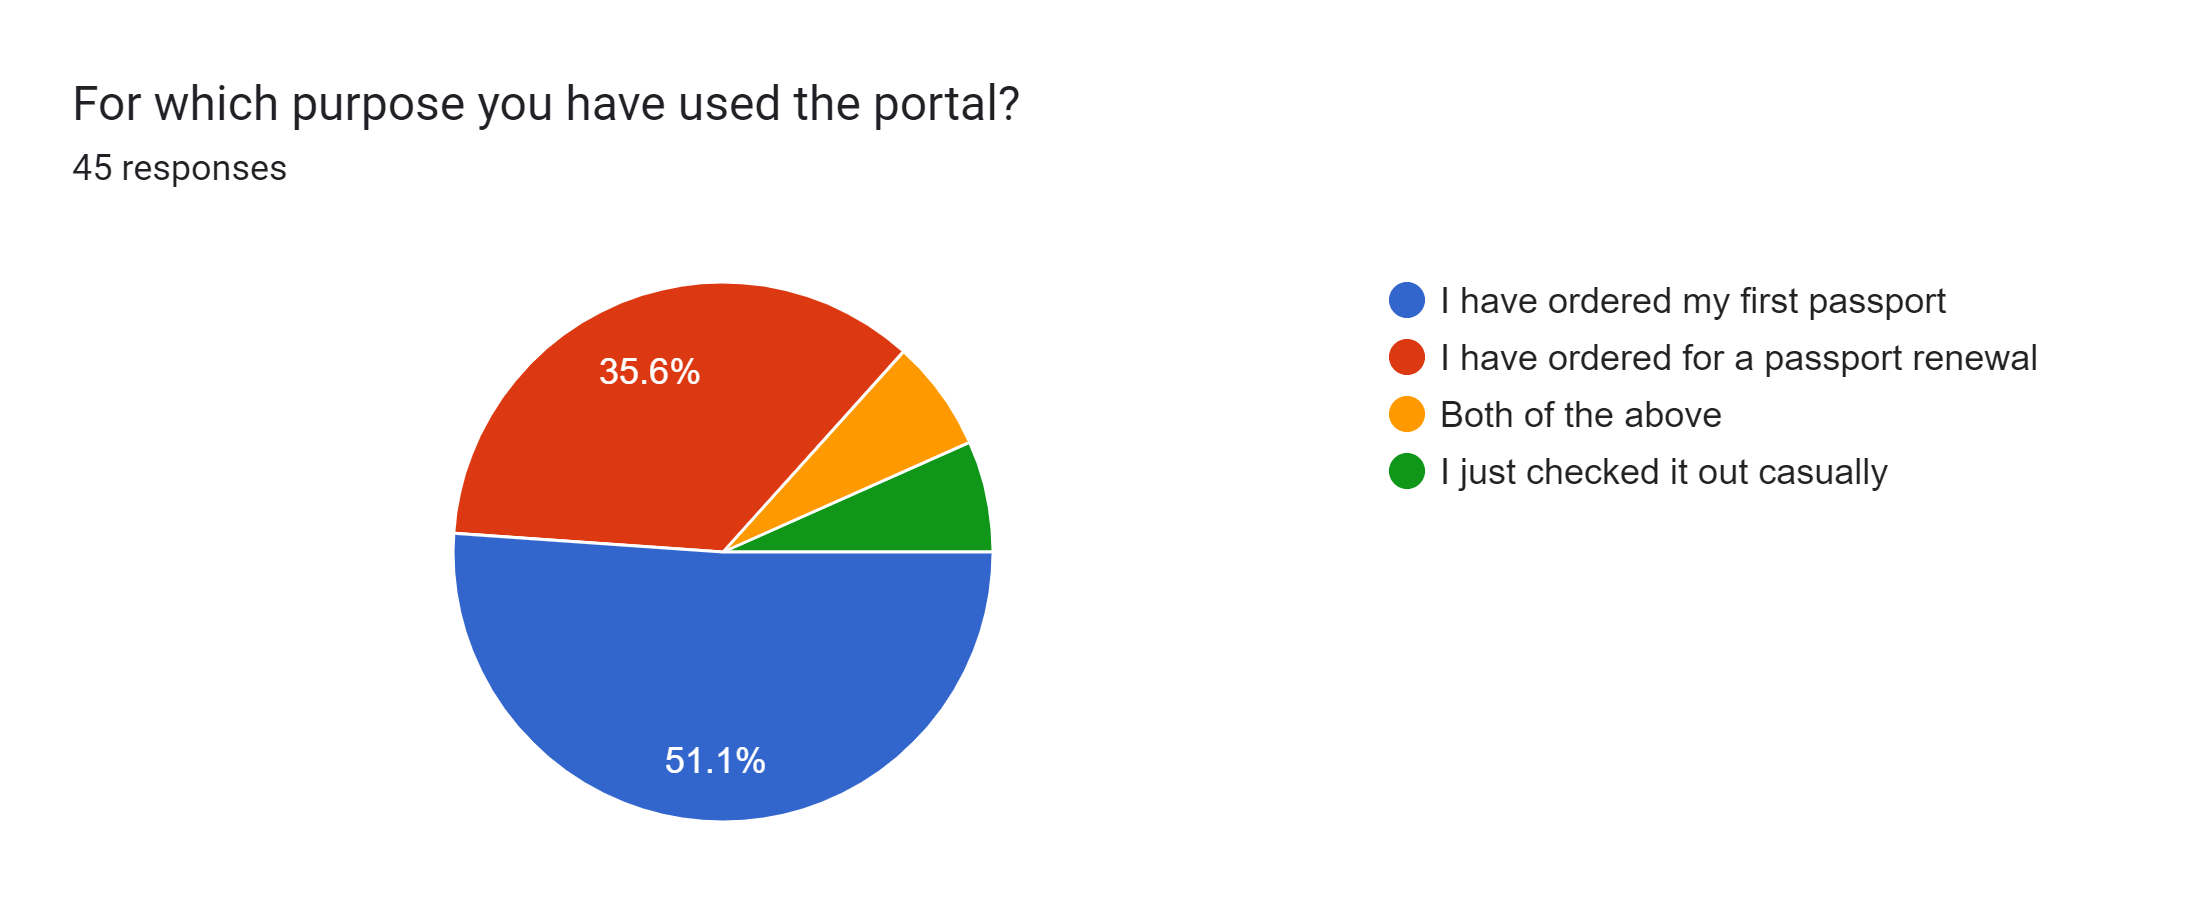
\includegraphics[width=\linewidth]{Figures/purpose.png}}
\vspace{-10pt}\caption{Percentage of users who faced issues related to user interface}
\label{fig:purpose}
\end{figure}

\subsection{Survey Response}

The second and more important set of findings came from other direct users of the system, through a questionnaire survey. Fig \ref{fig:purpose} shows that the users used the system for both applying for new passports and renewing expired passports. We present our findings in 5 categories described below:

\begin{figure}[ht]
\centering
\centerline{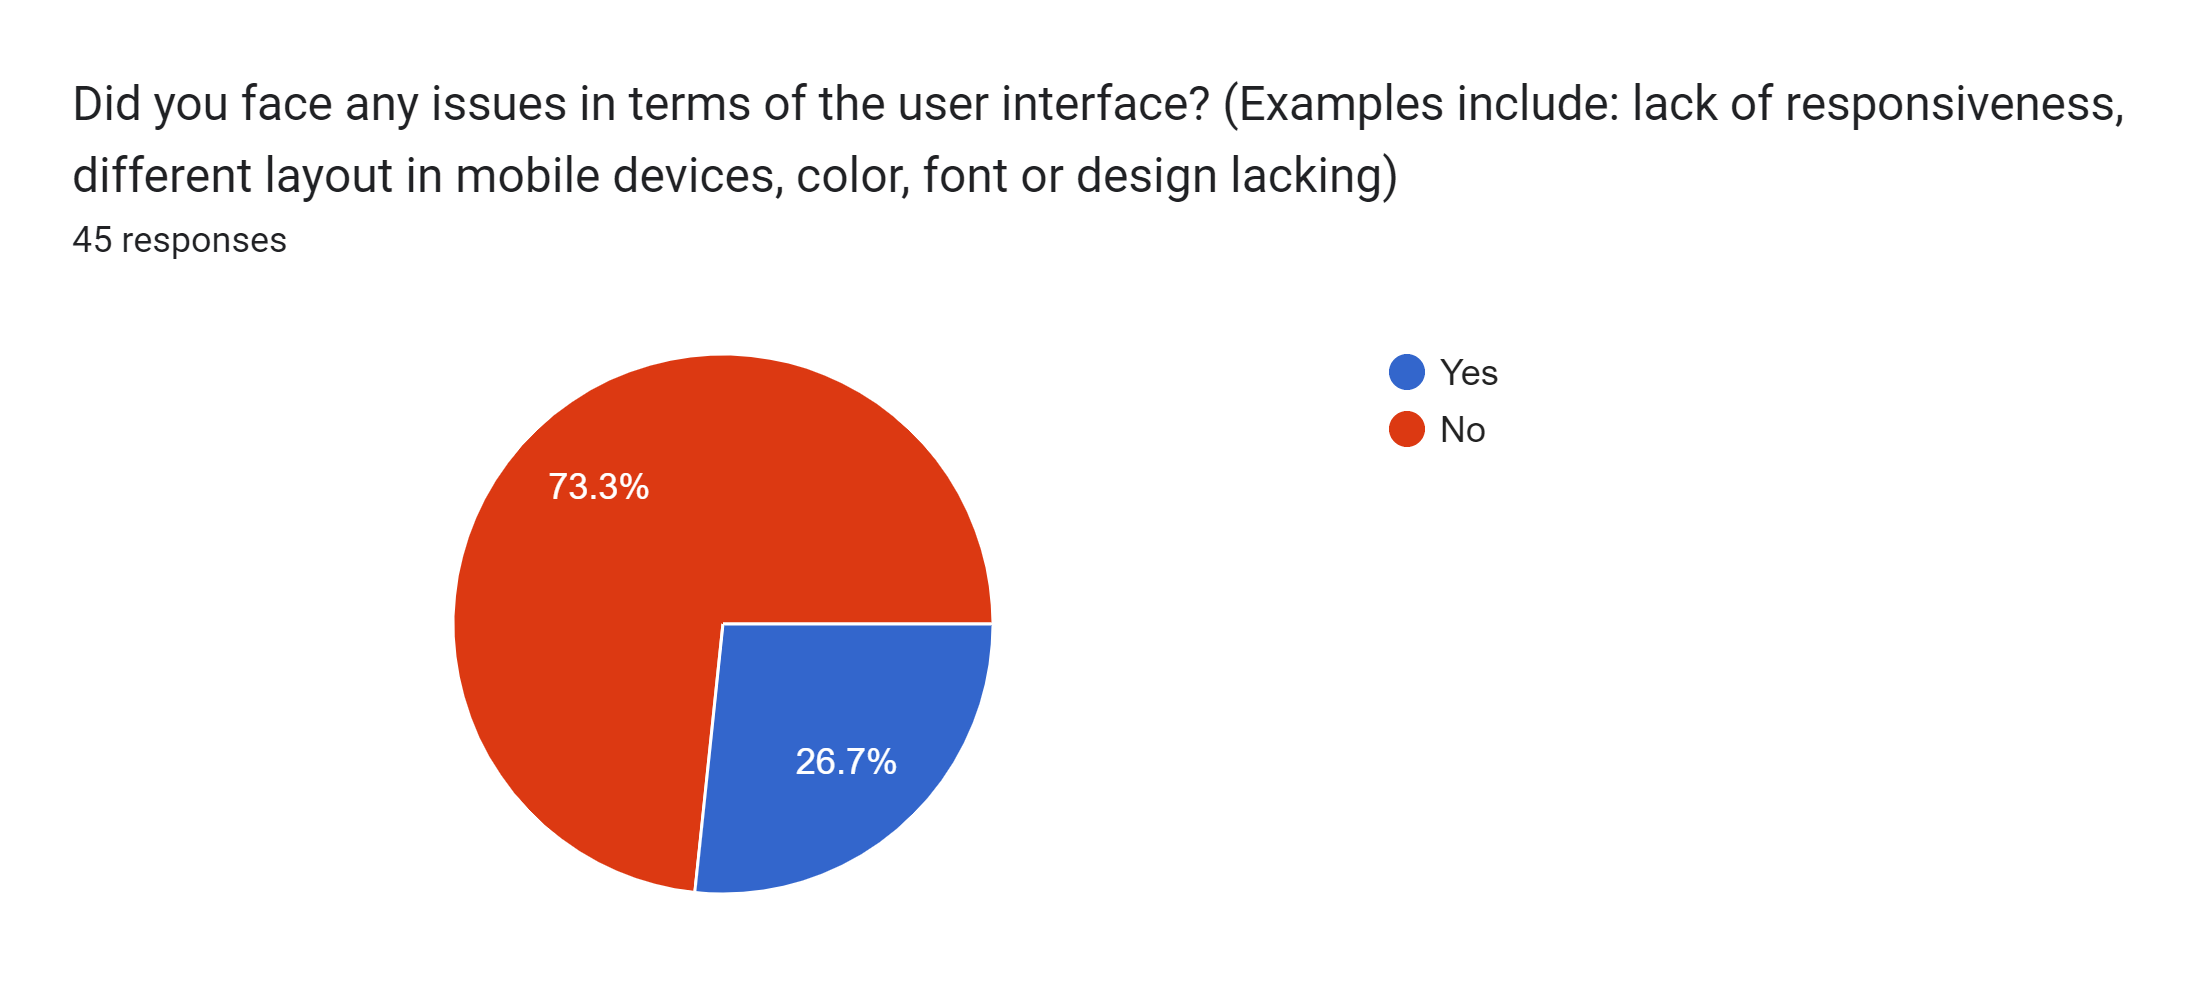
\includegraphics[width=\linewidth]{Figures/issueui.png}}
\vspace{-10pt}\caption{Reason of using e-Passport portal}
\label{fig:issueui}
\end{figure}

\subsubsection{UI Issues} 

The majority of the users shared that they found issues related to UI as pointed out by Fig: \ref{fig:issueui}. Some users faced problems while choosing a suitable interview date. According to their report, while looking for available interview dates, they got their calendar layer completely frozen. Some users let us know that they provided correct and valid information in the form yet got a submission error. Others commented that the UI seemed a bit unorganized, and navigating through the sections was difficult.
\newline

\subsubsection{Technical Issues}

Users had their complaints about the technical side of the website too \ref{fig:issuetech}. A couple of users reported that the 'One Time Password's (OTP) used for prompt verification appeared very late in some cases, hence leading to login and other procedural errors. Some also faced frequent captcha errors. Due to the high amount of system traffic, some of the users got automatically logged out after spending a little time logged in. Available appointment dates were found to be blank in some cases. Moreover, some users suggested that it would be great if there were options to edit or cancel the whole application even after submission in case of emergencies and get refunded, which is not currently available.

\begin{figure}[ht]
\centering
\centerline{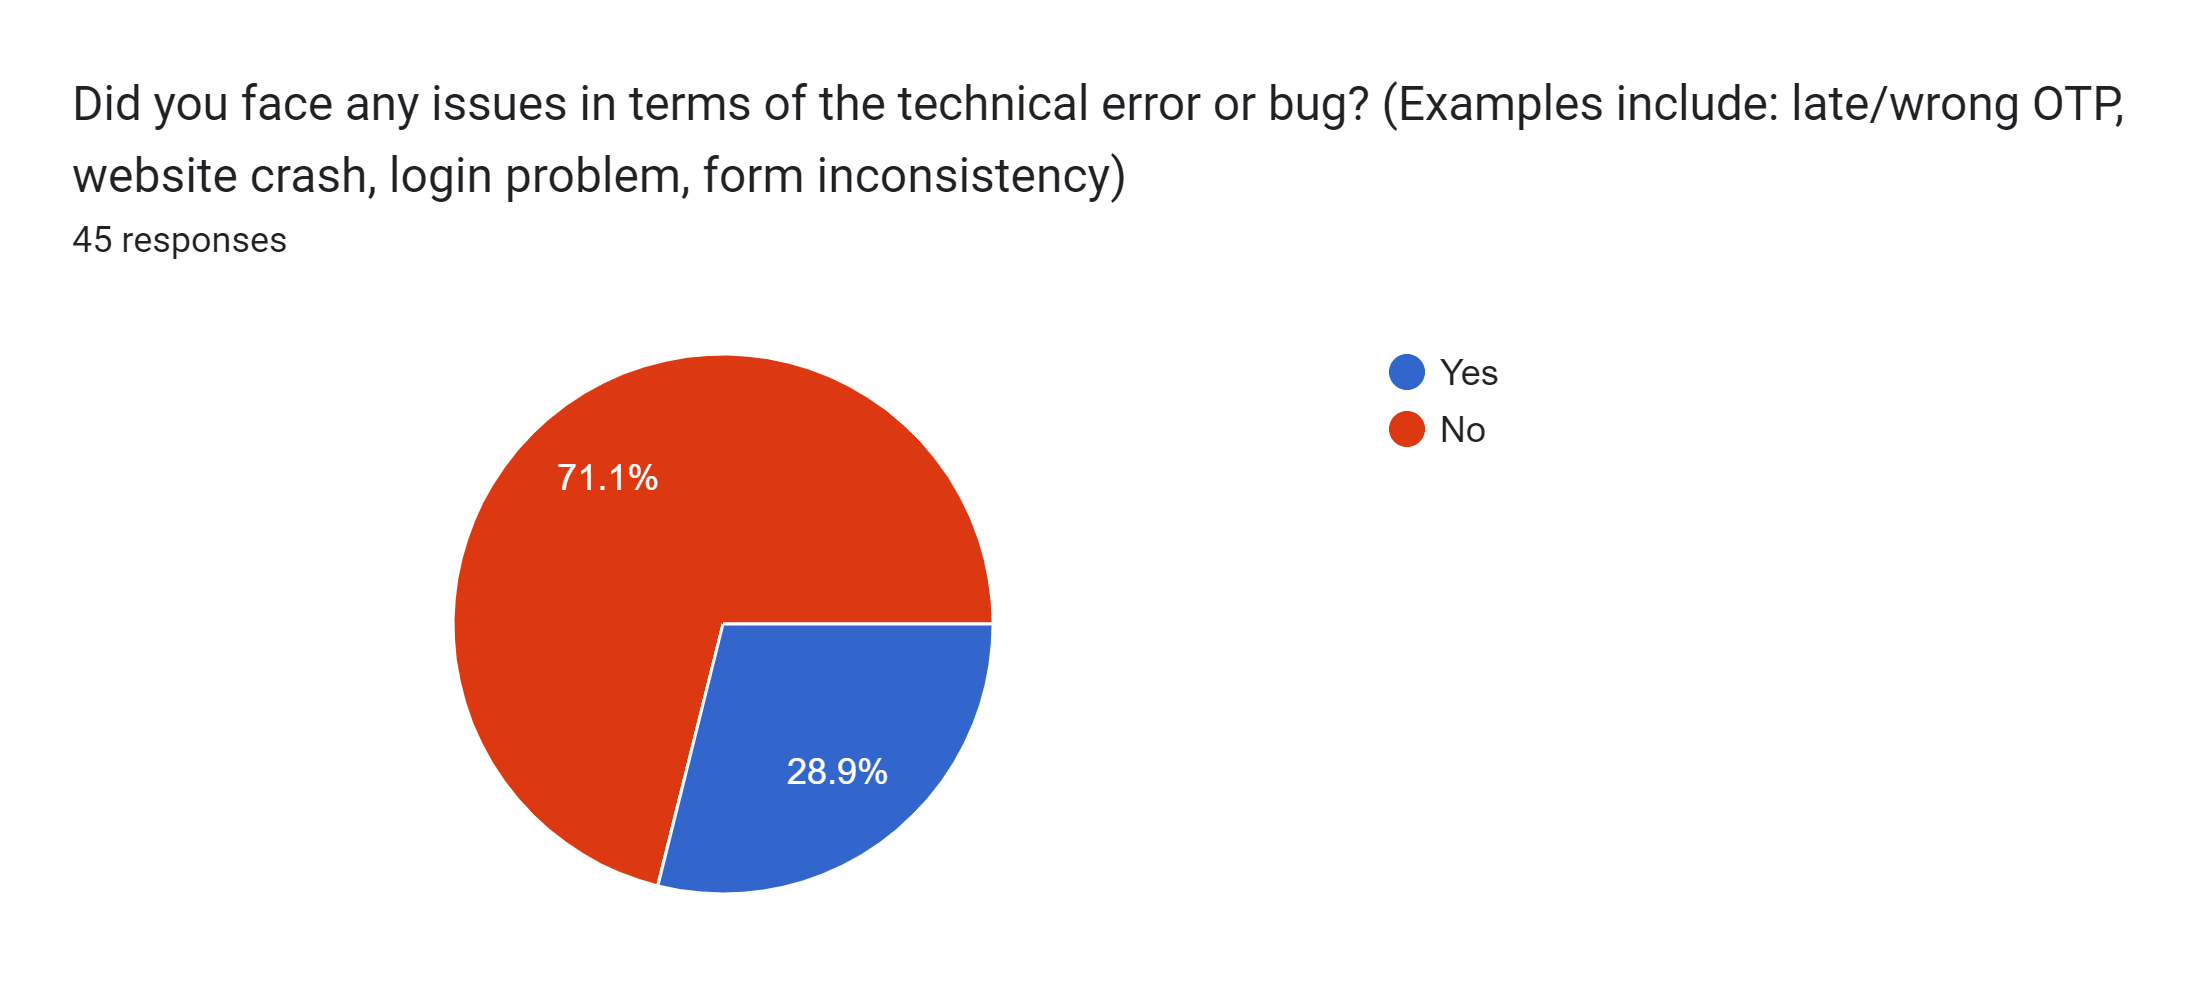
\includegraphics[width=\linewidth]{Figures/issuetech.png}}
\vspace{-10pt}\caption{Percentage of users who faced technical issues}
\label{fig:issuetech}
\end{figure}

A significant portion of the technical complaints was about the online payment system integrated with the website. Around 75.6\% of the users tried to do payments online \ref{fig:payment}, whereas almost 1/6th of the survey attendees mentioned that they could not use the online payment method as the service was down.

\begin{figure}[ht]
\centering
\centerline{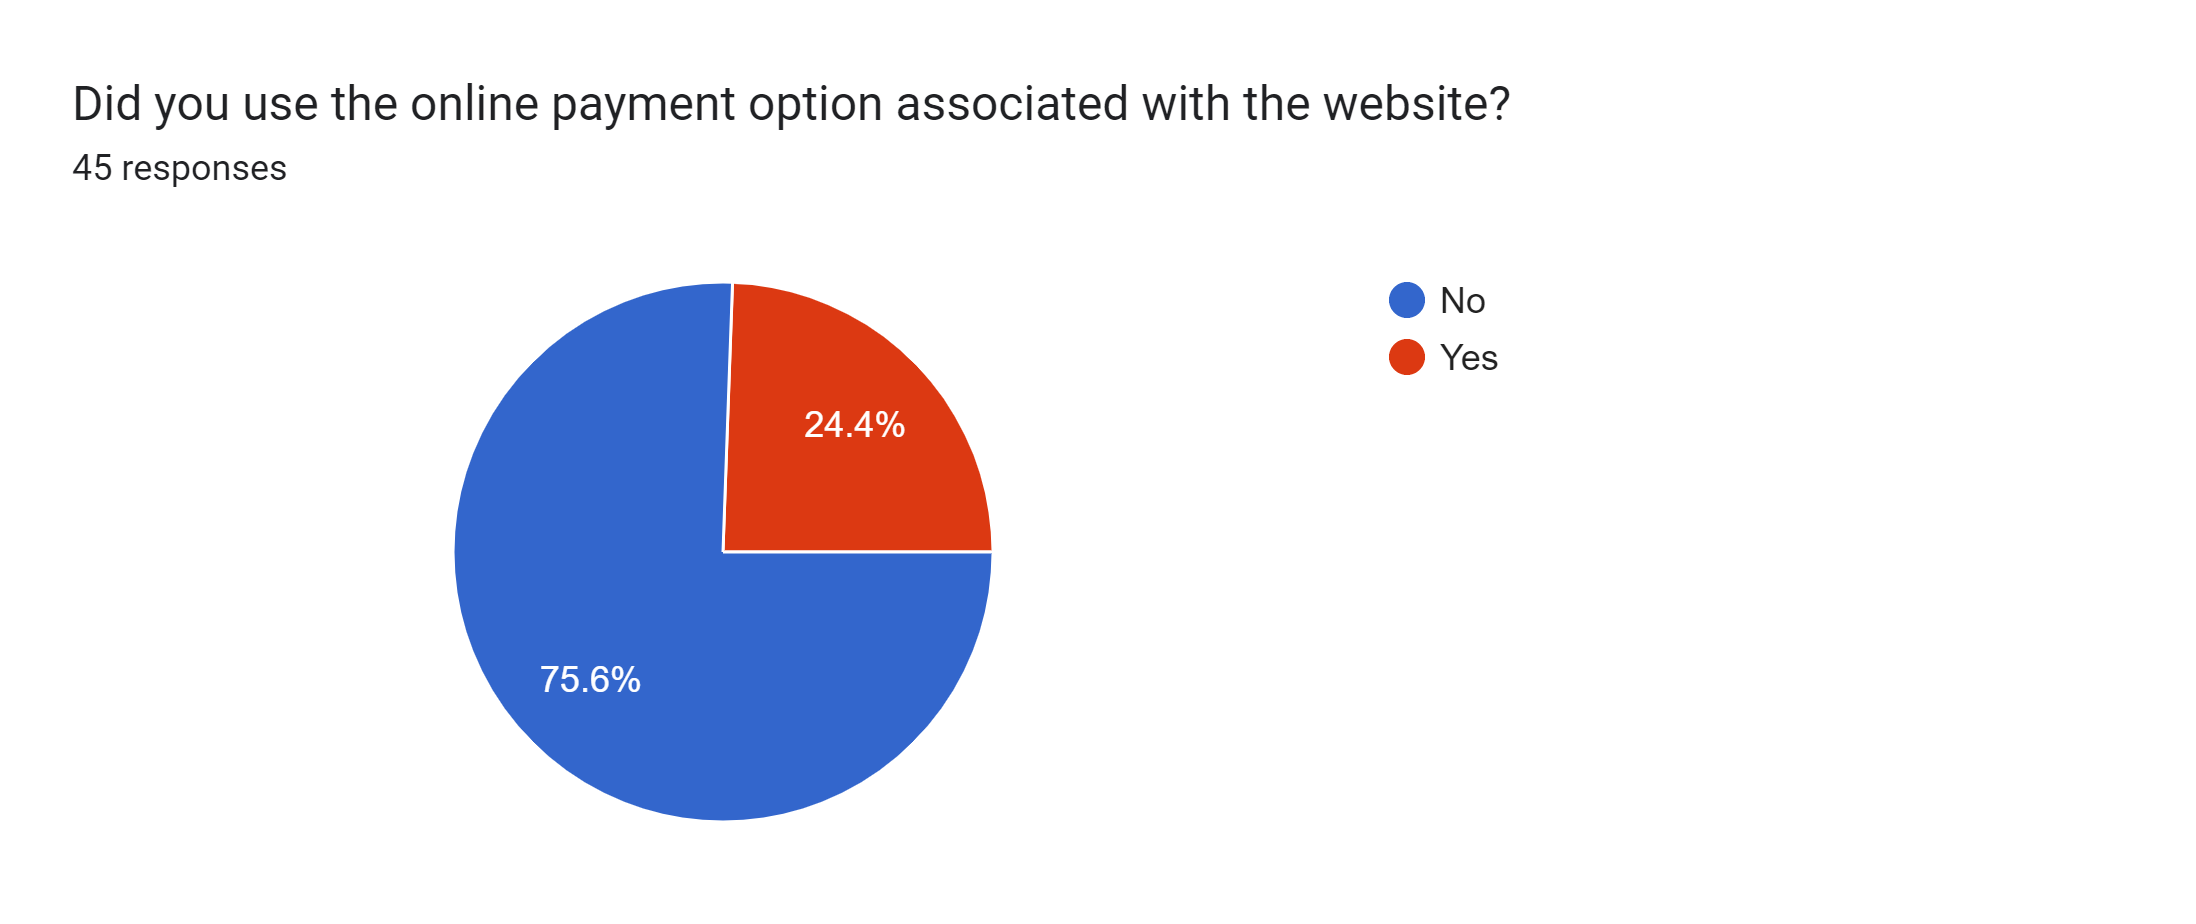
\includegraphics[width=\linewidth]{Figures/payment.png}}
\vspace{-10pt}\caption{Percentage of users who used the online payment module}
\label{fig:payment}
\end{figure}

A couple of clients had to undergo some errors during the payment, but they got their refund as well. One user also mentioned that the current E-Chalan online payment system is far worse than the previous Sonali bank system. The users also reported system crashes and UI freezing during the payment process. Some mentioned that the receipt download option after the confirmation was difficult to find. But apart from these issues, some users also shared that they did not face anything unpleasant while using the online payment.
\newline

\begin{figure}[ht]
\centering
\centerline{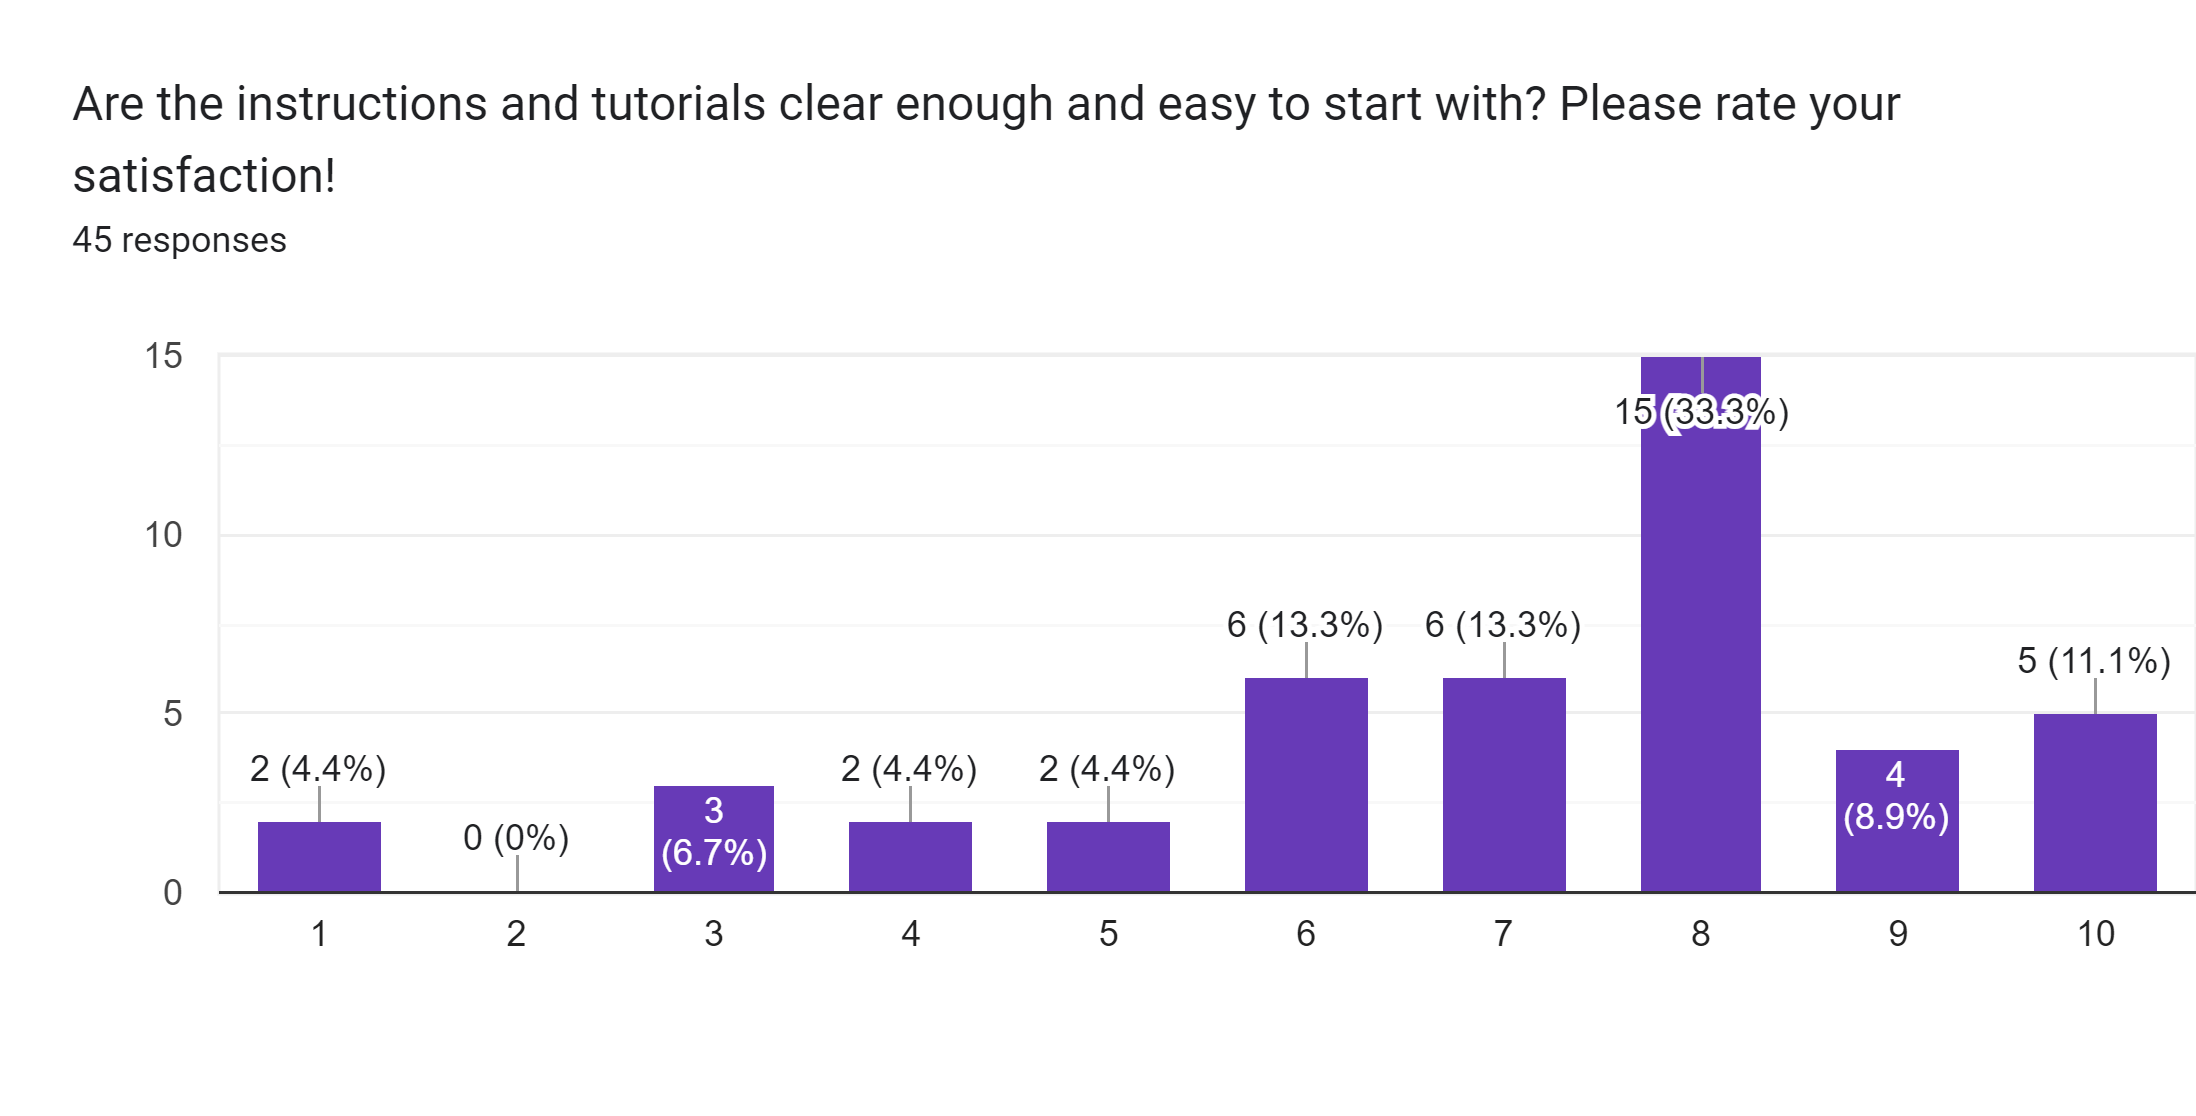
\includegraphics[width=\linewidth]{Figures/instructions.png}}
\vspace{-10pt}\caption{Bar chart showing satisfaction rating in terms of instruction and information clarity}
\label{fig:instruction}
\end{figure}

\subsubsection{Information Gap Issues}

Although most of the users found the information available just fine as per Fig \ref{fig:instruction} and \ref{fig:navigation}, some had their complaints and suggestions as well. The very frequent issue about the information gap the users faced is about no support for punctuation symbols like (.) and (:) in the user full name field. They suggested mentioning this explicitly around the form, otherwise, it was difficult to know whether these symbols were allowed or not. 


\begin{figure}[ht]
\centering
\centerline{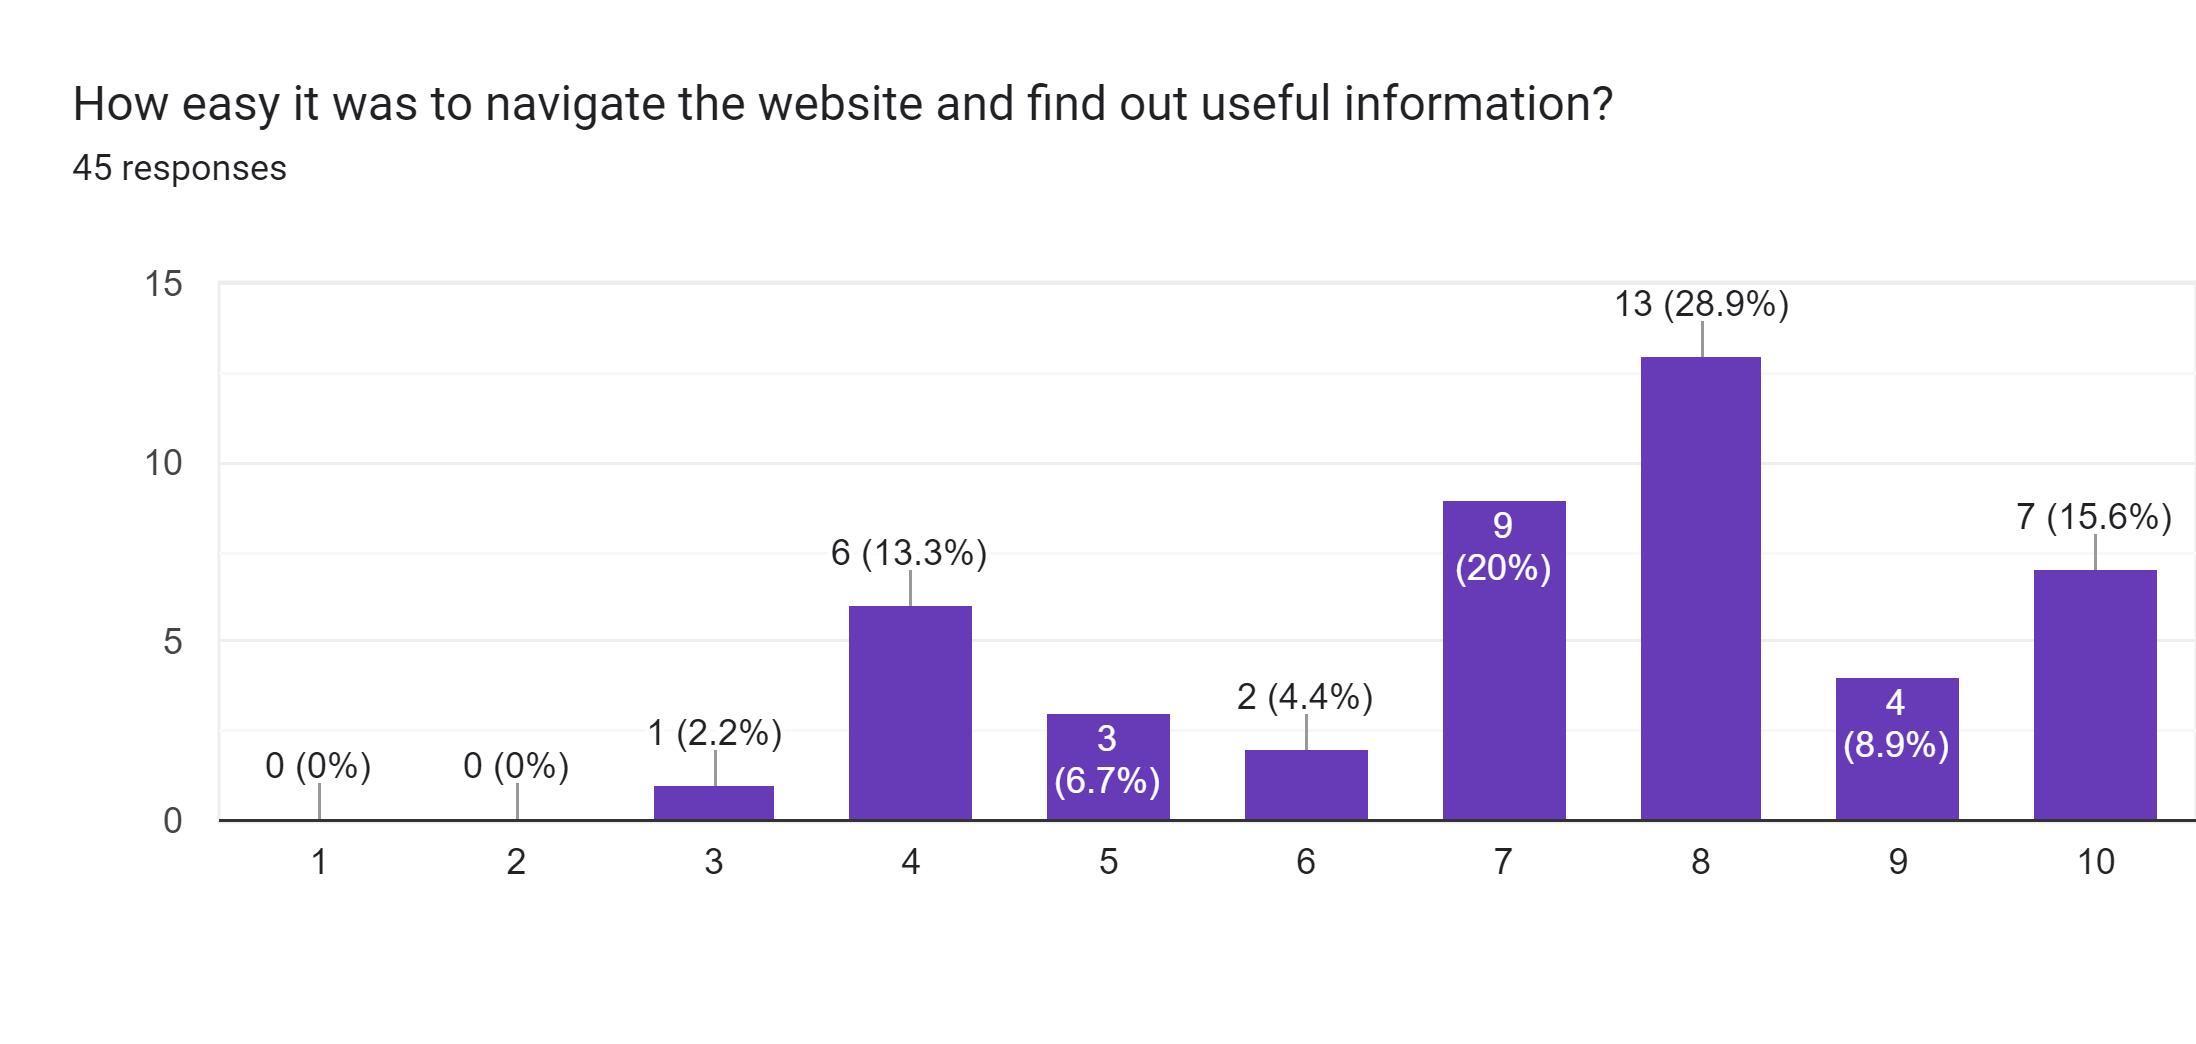
\includegraphics[width=\linewidth]{Figures/navigation.png}}
\vspace{-10pt}\caption{Bar chart showing satisfaction rating in terms of navigation and information}
\label{fig:navigation}
\end{figure}

As we, the authors found out earlier, some users reported that the document list that they needed to bring to the passport office, was not updated and correct on the website, which resulted in nothing but their additional suffering on the due date. Some users mentioned that some video tutorials could be of great help to new users.
\newline

\begin{figure}[ht]
\centering
\centerline{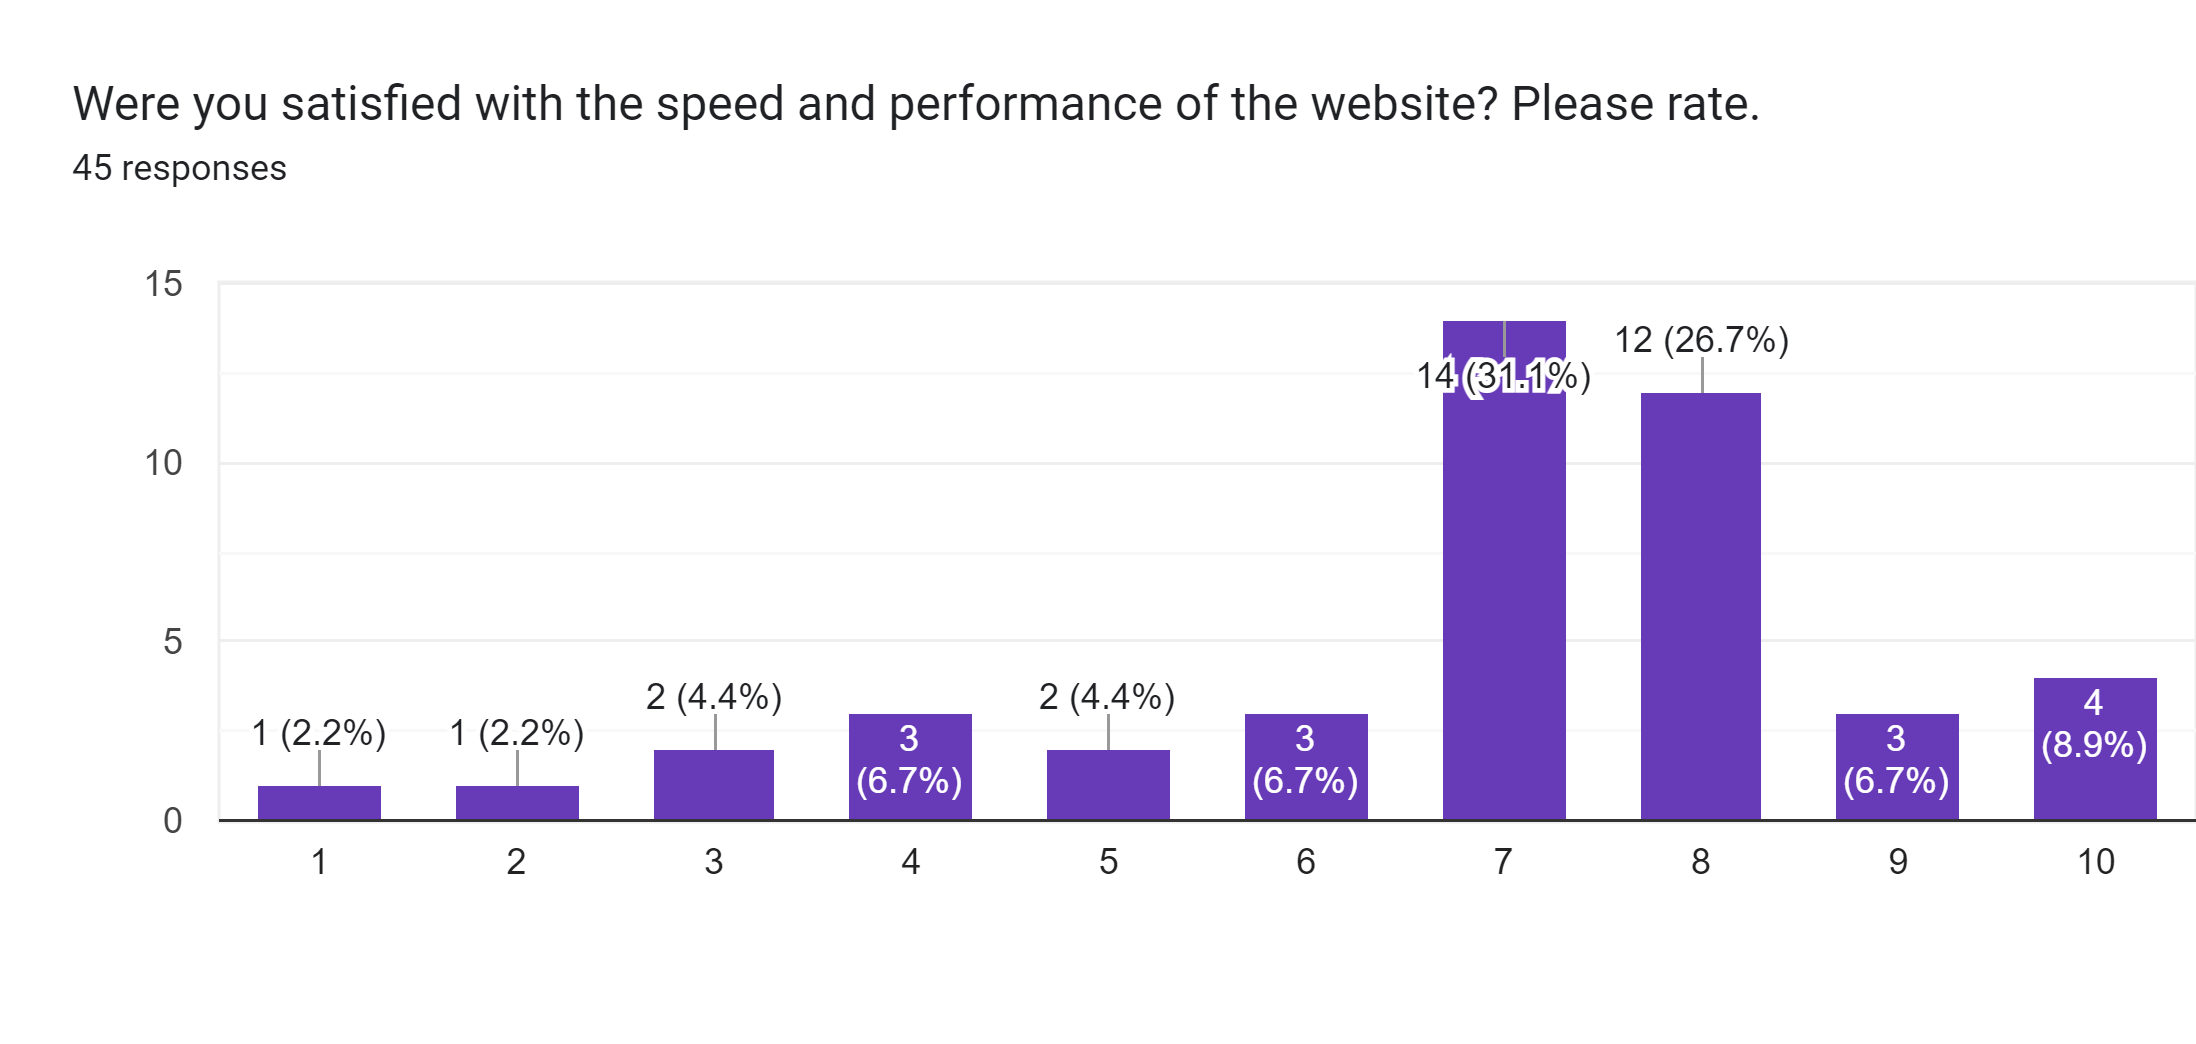
\includegraphics[width=\linewidth]{Figures/speed.png}}
\vspace{-10pt}\caption{Bar chart showing satisfaction rating in terms of speed and performance}
\label{fig:speed}
\end{figure}

\subsubsection{Performance Issues}

As it is quite clear from Fig \ref{fig:speed}, most of the users were quite satisfied with the speed of the software. However, some reported the slow response time of the system. 

Many of the users who already had an expired passport and applied for passport renewal through the website for the first time, shared a common concern. As it should be in a good online system, they were expecting their information to be already present in the database. Users were disappointed to fill up the same information again.
\newline

\subsubsection{Contact and Feedback Services}

Fig \ref{fig:contact} shows that just 13.3\% of the survey takers actually tried these services. Most of the users who tried to use the Contact services for further help reported that the module was not working, and they had to go to the offices physically. Hence, this module showed poor performance just like the payment module mentioned above.
\newline
\begin{figure}[ht]
\centering
\centerline{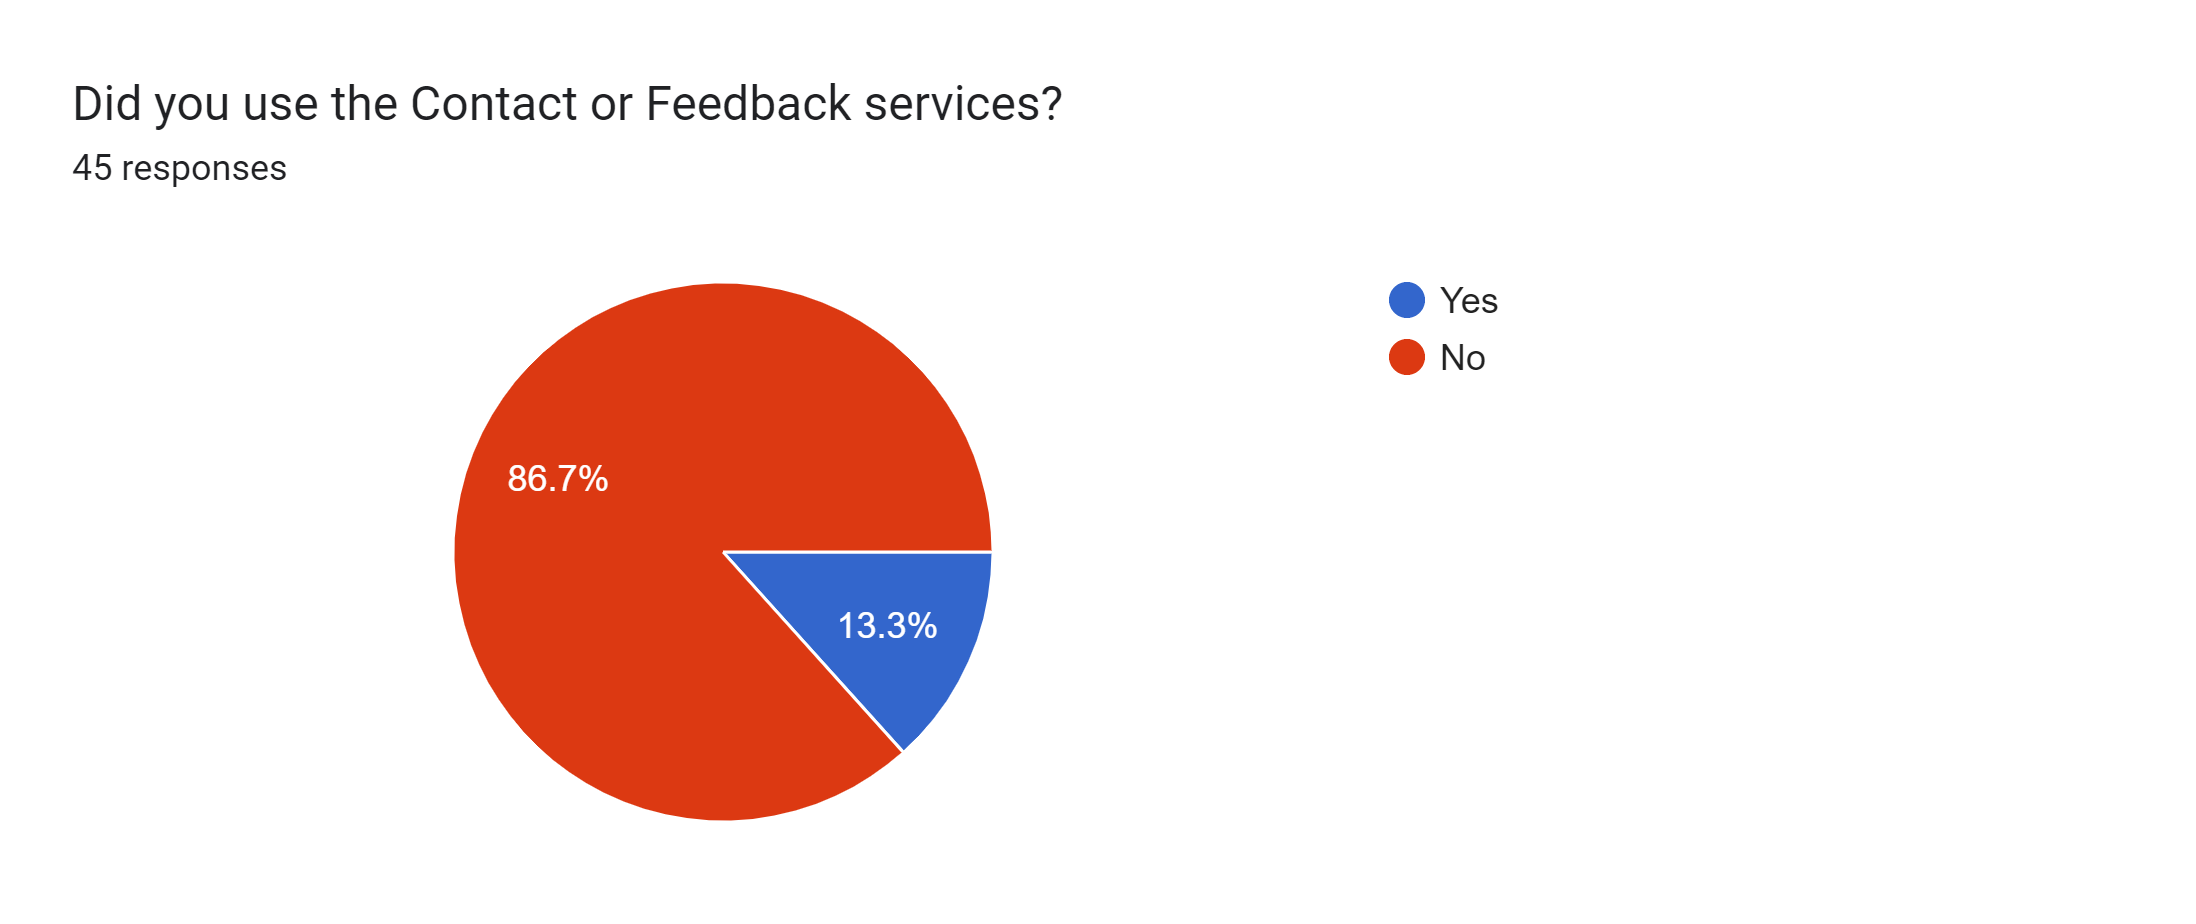
\includegraphics[width=\linewidth]{Figures/contact.png}}
\vspace{-10pt}\caption{Percentage of participants who used Contact or Feedback services}
\label{fig:contact}
\end{figure}

Finally, the users more or less liked the status tracking dashboard of the system as Fig \ref{fig:dash} shows.

\begin{figure}[ht]
\centering
\centerline{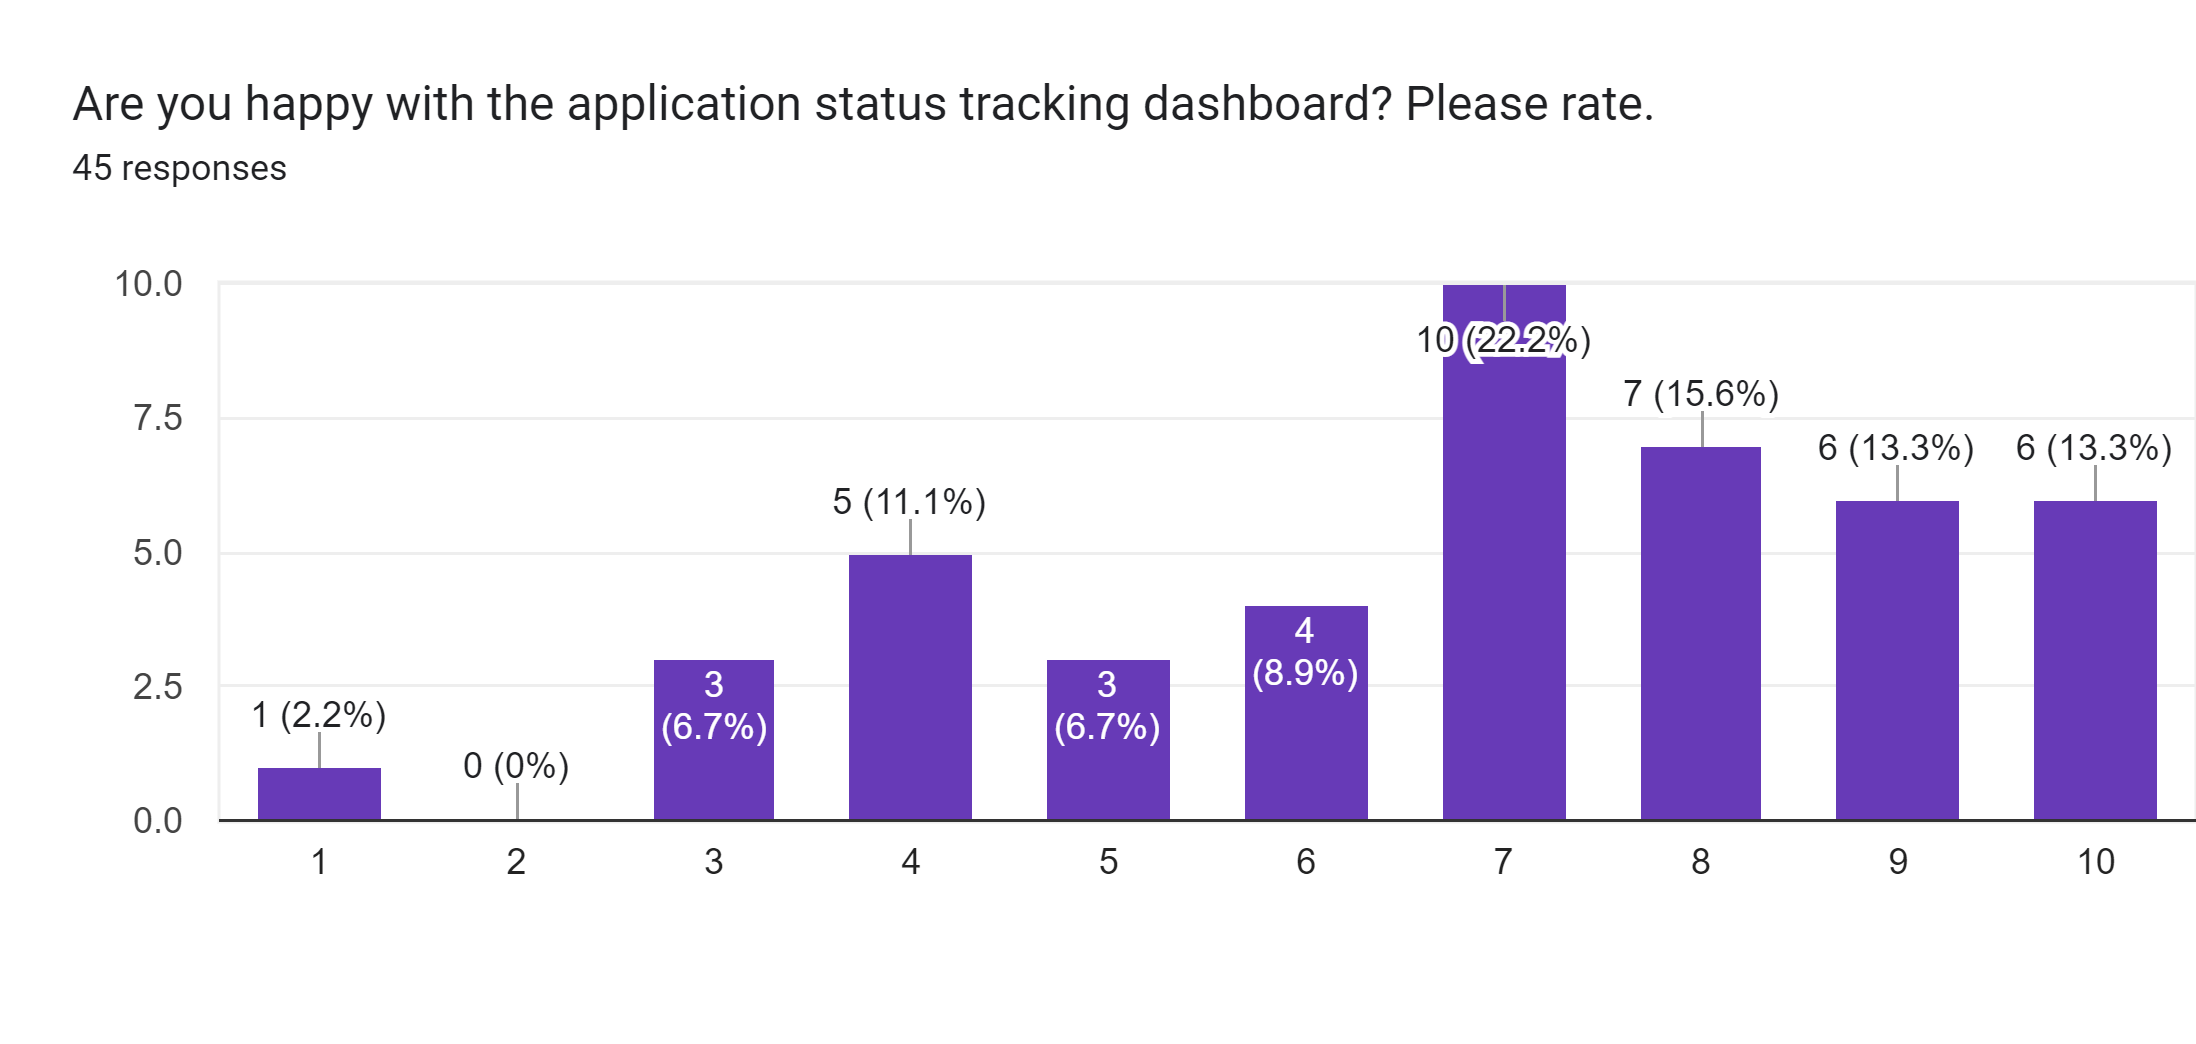
\includegraphics[width=\linewidth]{Figures/dashboard.png}}
\vspace{-10pt}\caption{User satisfaction rating for the application status dashboard}
\label{fig:dash}
\end{figure}

We summarize the positive and negative aspects of the website based on our findings in Table \ref{tab:summary}.

\begin{table*}[ht]
\centering
\caption{Positive and Negative Aspects of Bangladesh e-Passport Portal}
\label{tab:summary}
\begin{tabular}{cll}
\hline
% \begin{table}[ht]
% \begin{tabular}{\columnwidth}{@{\extracolsep{\fill}}}

\textbf{}&\textbf{Positive Aspects} & \textbf{Negative Aspects} \\\hline
1& Serves a huge population & Frequent login, logout and crashing errors\\
2&Status tracking dashboard is handy & Frequent OTP errors \\
3&No major inconsistency issue& Horrible payment module \\
4&Contains system feedback section & Updating, canceling, and refund flexibility needed \\
5&UI components are well-utilized and well-placed& Instructions need to get better \\
6&Offers simple error handling & Complaints about the unresponsiveness of the Contact section\\\hline
\end{tabular}
\end{table*}

\section{Recommendations and Conclusion}
\label{sec:discussion}

When prompted for an overall rating to provide to the system, the users mostly gave the web application 7 or 8 out 10, as Fig \ref{fig:overall} shows. However, a few suggestions came up from the survey, including introducing a passport home delivery system. Some of the users mentioned that the premium service fees were quite high.

\begin{figure}[ht]
\centering
\centerline{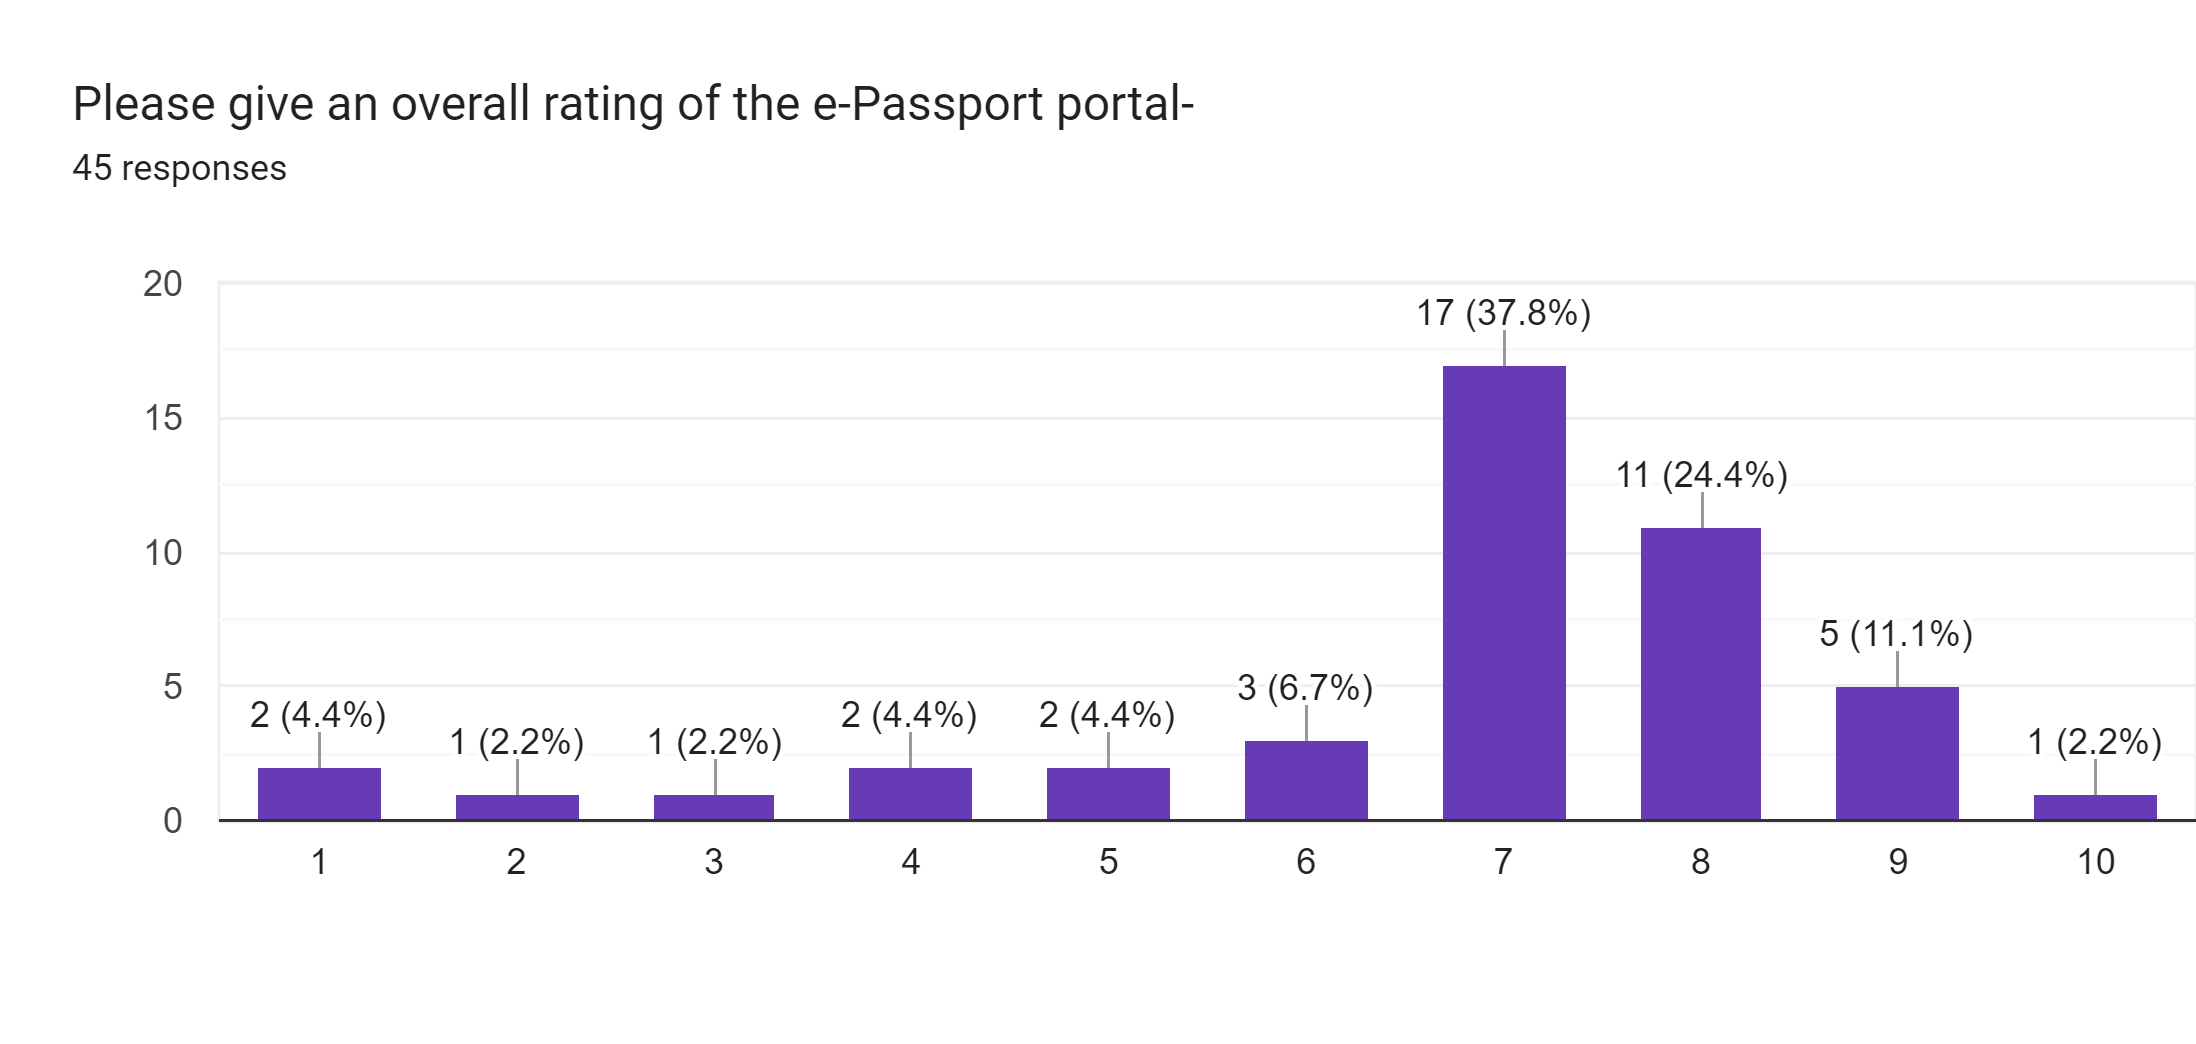
\includegraphics[width=\linewidth]{Figures/overall.png}}
\vspace{-10pt}\caption{Overall rating of the e-Passport portal}
\label{fig:overall}
\end{figure}

We present some suggestions based on the user feedback and 8 golden rules of interface design given by Shneiderman \cite{sp10}:

\begin{itemize}
    \item There should be enough flexibility regarding editing the application and even canceling it even after scheduling in case of emergencies. Easy reversal of actions should be permitted. 
    \item Focus must be increased on effective load balancing. Authorities might give thought to increasing the budget for skilled developers.
    \item The website should be updated on a regular basis to keep the information and instructions up-to-date and complete. 
    \item The payment module can be redesigned as the current one has been performing poorly for quite a period of time. 
    \item Video demonstrations of the application steps can be added to the homepage.
    \item Already existing database entries should be migrated carefully within the scope of the website so that renewal cases do not require filling up the same information again.
    \item Application progress summary can be shown in a sidebar as one proceeds through different sections of the form, effectively reducing the short-term of the user.
    \item The contact and feedback sections need to be improved. A dedicated help desk should be formed and monitored to be active. Feedback initiatives are recommended to be more frequent and to the point.
\end{itemize} 

Addressing the issues presented in this article will hopefully make the e-passport portal more user-friendly and effective enough to serve a large scale of people over the upcoming years.

% \input{Files/threats}
% \input{Files/relatedwork}
% \input{Files/conclusion}

\bibliographystyle{IEEEtran}
\bibliography{reference}

\end{document}
